% Oskar Weidner
\documentclass[../main.tex]{subfiles}
\graphicspath{{\subfix{../Abbildungen/}}}


\begin{document}
\renewcommand{\tasktitle}{Zwischen Quant, Band und Wand} % texorpdfstring wird in Titeln und Captions verwendet, wenn Zeichen verwendet werden, die so im Inhaltsverzeichnis nicht darstellbar sind; normalerweise weisen Aufgabentitel keine Fussnote auf
\renewcommand{\taskpoints}{28.5} %Gesamtpunktzahl der Aufgabe
\renewcommand{\taskweight}{9000}
\aufgabenanfang% Beginn der Aufgabe

Die Energie einer chemischen Bindung hängt vom Abstand der beteiligten Atome ab. Aus dem Verlauf dieser Energie lassen sich verschiedene Eigenschaften der Bindung ableiten. Als eine Möglichkeit, um diesen Energieverlauf zu beschreiben, wird das sogenannte Morse-Potential genutzt:
\begin{align}
    V_{\text{Morse}}(r) &= D_e \cdot \left(1-e^{-a\cdot(r-r_e)}\right)^2\label{morse}
\end{align}
Der Parameter $a$ beschreibt dabei die Breite der Potentialfunktion.
\teilaufgabe{\operator{Vervollständige} die Achsenbeschriftung im Diagramm und markiere die Gleichgewichts-Bindungslänge \(r_\text{e}\) sowie die Bindungsenergie \(D_e\).\punkte{3}}{}
\kasten{100mm}{
\begin{figure}[H]
    \centering
    \opt{0}{\begin{tikzpicture}
\begin{axis}[
    width=12cm, height=9cm,
    xmin=0.55, xmax=3.65,
    ymin=-1, ymax=16.2,
    xtick={1,2,3},
    ytick={0,5,10,15},
    tick align=outside,
    tick style={black, thin},
    axis line style={black, thin},
    clip=true,
    minor tick num=0,
    xticklabel style={font=\normalsize},
    yticklabel style={font=\normalsize},
]
% Morse-Potential: V(r) = D_e * (1 - exp(-a(r-r_e)))^2
% D_e = 11, r_e = 1.1, a = 2.35
\addplot[domain=0.55:3.65, samples=300, black, thick] {11*(1-exp(-2.35*(x-1.1)))^2};
\node[right] at (axis cs:0.8,15) {$V_{\text{Morse}}(r)$};
\end{axis}
\end{tikzpicture}}
    \opt{1}{\begin{tikzpicture}
\begin{axis}[
    width=12cm, height=9cm,
    xmin=0.55, xmax=3.65,
    ymin=-1, ymax=16.2,
    xtick={1,2,3},
    ytick={0,5,10,15},
    tick align=outside,
    tick style={black, thin},
    axis line style={black, thin},
    clip=true,
    minor tick num=0,
    xticklabel style={font=\normalsize},
    yticklabel style={font=\normalsize},
    xlabel={\textcolor{red}{Abstand $r$ (0.5P)}},
    ylabel={\textcolor{red}{Energie $E$ bzw. Potential $V$ (0.5P)}},
    xlabel style={red},
    ylabel style={red},
    extra x ticks={1.1},
    extra x tick labels={$r_e$ (1P)},
    extra x tick style={
        tick style={red, thin},
        tick label style={red, yshift=-8pt},
    },
    extra y ticks={11.1},
    extra y tick labels={$D_e$ (1P)},
    extra y tick style={
        tick style={red, thin},
        tick label style={red, xshift=-2pt},
    },
]
% Morse-Potential: V(r) = D_e * (1 - exp(-a(r-r_e)))^2
% D_e = 11, r_e = 1.1, a = 2.35
\addplot[domain=0.55:3.65, samples=300, black, thick] {11*(1-exp(-2.35*(x-1.1)))^2};
\node[right] at (axis cs:0.8,15) {$V_{\text{Morse}}(r)$};
 
% Hilfslinien zu r_e und D_e (rot, gestrichelt)
\draw[red, dashed, thin] (axis cs:1.1,-1) -- (axis cs:1.1,0);
\draw[red, dashed, thin] (axis cs:0.55,11.1) -- (axis cs:3.65,11.1);
\end{axis}
\end{tikzpicture}}
    \opt{2}{\begin{tikzpicture}
\begin{axis}[
    width=12cm, height=9cm,
    xmin=0.55, xmax=3.65,
    ymin=-1, ymax=16.2,
    xtick={1,2,3},
    ytick={0,5,10,15},
    tick align=outside,
    tick style={black, thin},
    axis line style={black, thin},
    clip=true,
    minor tick num=0,
    xticklabel style={font=\normalsize},
    yticklabel style={font=\normalsize},
    xlabel={\textcolor{red}{Abstand $r$ (0.5P)}},
    ylabel={\textcolor{red}{Energie $E$ bzw. Potential $V$ (0.5P)}},
    xlabel style={red},
    ylabel style={red},
    extra x ticks={1.1},
    extra x tick labels={$r_e$ (1P)},
    extra x tick style={
        tick style={red, thin},
        tick label style={red, yshift=-8pt},
    },
    extra y ticks={11.1},
    extra y tick labels={$D_e$ (1P)},
    extra y tick style={
        tick style={red, thin},
        tick label style={red, xshift=-2pt},
    },
]
% Morse-Potential: V(r) = D_e * (1 - exp(-a(r-r_e)))^2
% D_e = 11, r_e = 1.1, a = 2.35
\addplot[domain=0.55:3.65, samples=300, black, thick] {11*(1-exp(-2.35*(x-1.1)))^2};
\node[right] at (axis cs:0.8,15) {$V_{\text{Morse}}(r)$};
 
% Hilfslinien zu r_e und D_e (rot, gestrichelt)
\draw[red, dashed, thin] (axis cs:1.1,-1) -- (axis cs:1.1,0);
\draw[red, dashed, thin] (axis cs:0.55,11.1) -- (axis cs:3.65,11.1);
\end{axis}
\end{tikzpicture}}
\end{figure}
}{}

Das Morse-Potential beschreibt zwar die energetischen Verhältnisse der Bindung sehr gut, ist zum Rechnen jedoch aufgrund der relativ komplexen Formel häufig nicht geeignet. Um das Rechnen zu vereinfachen kann eine harmonische Näherung getroffen werden. Dabei wird die Bindung als einfacher Federschwinger angenommen, dessen Potential wie folgt berechnet wird:
\begin{align}
    V_\text{harmonisch}(r) &= \frac{1}{2} k \cdot (r-r_e)^2\quad\text{mit }k=2D_e\cdot a^2
\end{align}
Die Bindungsenergie kann zwar durch das harmonische Potential nicht mehr beschrieben werden, stattdessen wird jedoch die Kraftkonstante \(k\) eingeführt, welche im makroskopischen Kontext einer Federkonstante entsprechen würde.

\teilaufgabe{\operator{Kreuze an}, ob die folgenden Aussagen über Bindungen und Kraftkonstanten richtig oder falsch sind.\punkte{3}}{}
\MCvrfAnfang
\MCv{o}{Für Bindungen mit größeren Kraftkonstanten ist die maximale Auslenkung der Bindung höher.}
\MCv{x}{Bindungen mit kleineren Kraftkonstanten sind meist länger.}
\MCv{x}{Die \ch{C-C}-Bindung in Ethin hat eine größere Kraftkonstante als die in Ethan.}
\MCv{o}{Kürzere Bindungen haben generell eine kleinere Bindungsenergie.}
\MCv{x}{Kohlenstoffmonoxid hat eine größere Bindungsenergie $D_e$ als Kohlenstoffdioxid}
\MCv{o}{Doppelbindungen sind leichter zu brechen als Einfachbindungen.}
\MCvrfEnde

Unter Verwendung der Schrödingergleichung kann unter Nutzung des harmonischen Potentials die folgende Gleichung für die Energie aller möglichen Schwingungszustände einer Bindung hergeleitet werden:
\begin{align}
    E_n = \hbar\cdot\omega\cdot\left(n+\frac{1}{2}\right)\quad\text{mit }\omega = \sqrt{\frac{k}{\mu}}\text{ und }\mu=\frac{m_1\cdot m_2}{m_1+m_2}
\end{align}
Hier wurde die Schwingungsquantenzahl \(n\) eingeführt. Bei quantenchemischen Energieübergängen (wie bspw. die Absorption eines Photons) gilt für diese:
\begin{align}
    \Delta n = \pm1
\end{align}
Für die sogenannte Nullpunktsenergie, also die minimale Energie der Schwingung, ergibt sich also
\begin{align}
    E_0 &= \frac{1}{2}\hbar\cdot\omega\;.
\end{align}

Für die Absorption eines Photons ergibt sich nach der Auswahlregel $\Delta n=\pm 1$ für dessen Wellenzahl die Formel
\begin{align}\label{eq:nu_Ph}
    \tilde\nu_{Ph} &= \frac{1}{2\pi\cdot c}\cdot \sqrt{\frac{k}{\mu}}\;.
\end{align}

\teilaufgabe{\operator{Leite} die \autoref{eq:nu_Ph} \operator{her}.}{Es gilt allgemein \(\tilde\nu = \frac{1}{\lambda}\) und \(\hbar = \frac{h}{2\pi}\).}
\kasten{75mm}{
    \begin{align*}
        \Delta E &= E_{n+1} - E_n\punkte{0.5}\\
        &= \hbar\cdot\omega\cdot\left(n + 1 +\frac{1}{2}\right) - \hbar\cdot\omega\cdot\left(n+\frac{1}{2}\right)\\
        &= \hbar\cdot\omega\punkte{1}\\
        \Delta E &= E_{Ph} \punkte{1}\\
        &= h \cdot \frac{c}{\lambda_{Ph}} = h\cdot c\cdot\tilde\nu_{Ph} \punkte{0.5}\\
        \Rightarrow \tilde\nu_{Ph} &= \frac{\Delta E}{h\cdot c}\punkte{0.5}\\
        &= \frac{\frac{h}{2\pi} \cdot \sqrt{\frac{k}{\mu}}}{h\cdot c} = \frac{1}{2\pi \cdot c} \cdot \sqrt{\frac{k}{\mu}}\punkte{1}
    \end{align*}
}{}

In der Astrochemie werden mitunter durch spektroskopische Methoden die Zusammensetzungen verschiedener stellarer Objekte untersucht. So konnte beispielsweise die Präsenz von Kohlenstoffmonoxid im interstellaren Raum über Infrarotspektroskopie (IR-Spektroskopie) nachgewiesen werden. Dabei wurde eine Bande mit einer Wellenzahl von \SI{2143}{\per\centi\metre} observiert.

\teilaufgabe{\operator{Berechne} die Kraftkonstante der angeregten Kohlenstoffmonoxidschwingung, die im IR-Spektrum beobachtet werden konnte.}{}
\kasten{80mm}{
    \begin{align*}
        \tilde\nu_{Ph} &= \frac{1}{2\pi\cdot c}\cdot\sqrt{\frac{k}{\mu}}\punkte{0.5}\\
        \Rightarrow k &= \left(\tilde\nu_{Ph}\cdot2\pi\cdot c\right)^2\cdot\mu_{\ch{CO}}\punkte{0.5}\\
        \mu_{\ch{CO}} &= \frac{m_{\ch{C}}\cdot m_{\ch{O}}}{m_{\ch{C}} + m_{\ch{O}}} = \frac{\SI{12.011}{\atomicmassunit} \cdot \SI{15.999}{\atomicmassunit}}{\SI{12.011}{\atomicmassunit}+\SI{15.999}{\atomicmassunit}} = \SI{6.861}{\atomicmassunit}\punkte{1}\\
        k &= \left(\SI{214300}{\per\metre}\cdot2\pi\cdot \SI{2.998e8}{\metre\per\second}\right)^2\cdot\num{6.861}\cdot\SI{1.661e-27}{\kilo\gram}\punkte{1}\\
        &= \SI{1801}{\newton\per\metre}\punkte{1}
    \end{align*}
}{}

Zur Bestätigung des Vorliegens von zwei Chlorisotopen (\ch{^{35}Cl} und \ch{^{37}Cl}) wurde ein IR-Spektrum von \ch{HCl_{(g)}} aufgenommen. Dieses zeigte für die untersuchte Streckschwingung die Wellenzahlen \SI{2883.8}{\per\cm} und \SI{2886.0}{\per\cm} auf.
\newpage
\teilaufgabe{\operator{Untersuche rechnerisch}, ob tatsächlich \ch{^{35}Cl} und \ch{^{37}Cl} vorliegen.}{Gehe dabei für alle beteiligten Atome von ganzzahligen atomaren Massen aus.}
\kasten{110mm}{
Weisen beide Schwingungen für die Isotopen jeweils die gleiche Kraftkonstante auf, können die Massenzahlen bestätigt werden.\punkte{1}
Das schwerere Isotop liefert die kleinere Wellenzahl. \kommentar{Muss nicht explizit gesagt werden, reicht auch einfach so zu nutzen oder alle Möglichkeiten durchzurechnen.}\punkte{0.5}
Verschiedene Lösungswege sind möglich, beispielsweise:
    \begin{align*}
        k_1 &= \left(\tilde\nu_{\ch{H^{35}Cl}}\cdot2\pi\cdot c\right)^2\cdot\mu_{\ch{H^{35}Cl}}\\
        &= \left(\SI{288600}{\per\metre} \cdot2\pi\cdot \SI{2.998e8}{\metre\per\second}\right)^2\cdot\frac{35}{36}\cdot\SI{1.661e-27}{\kilo\gram}=\SI{477.26}{\newton\per\metre}\\
        k_2 &= \left(\tilde\nu_{\ch{H^{37}Cl}}\cdot2\pi\cdot c\right)^2\cdot\mu_{\ch{H^{37}Cl}}\\
        &= \left(\SI{288380}{\per\metre} \cdot2\pi\cdot \SI{2.998e8}{\metre\per\second}\right)^2\cdot\frac{37}{38}\cdot\SI{1.661e-27}{\kilo\gram}=\SI{477.24}{\newton\per\metre}
    \end{align*}
oder
    \begin{align*}
        \frac{\tilde\nu_{\ch{H^{35}Cl}}}{\tilde\nu_{\ch{H^{37}Cl}}}
    	&= \frac{2\pi\cdot c\cdot\sqrt{k\cdot\mu_{\ch{H^{37}Cl}}}}{
            2\pi\cdot c\cdot\sqrt{k\cdot\mu_{\ch{H^{35}Cl}}}}
    	=\sqrt{\frac{\mu_{\ch{H^{37}Cl}}}{\mu_{\ch{H^{35}Cl}}}}\\
        \Rightarrow\tilde\nu_{\ch{H^{35}Cl}} &= \sqrt{\frac{\mu_{\ch{H^{37}Cl}}}{\mu_{\ch{H^{35}Cl}}}}\cdot\tilde\nu_{\ch{H^{37}Cl}} = \sqrt{\frac{\sfrac{37}{38}}{\sfrac{35}{36}}}\cdot\SI{2883.8}{\per\centi\metre}=\SI{2886}{\per\cm}
    \end{align*}
\ch{^{35}Cl} und \ch{^{37}Cl} sind damit bestätigt.\punkte{1} \kommentar{Folgefehlerbepunktung bei kleineren Fehlern in der Rechnung möglich}

\kommentar{auf richtige Rechnung, egal wie gemacht\punkte{2}; Teilpunkte möglich}
}{}

Auch andere Systeme können relativ einfach quantenchemisch beschrieben werden. So kann beispielsweise mit dem Konzept des Teilchens im Kasten die Energie approximiert werden, die konjugierte Systeme absorbieren können. Man nimmt dabei an, dass das betrachtete Elektron in einem sogenannten Potentialtopf gefangen ist. Das bedeutet, dass sich das Teilchen nur in einem bestimmten Längenbereich $L$ aufhalten kann, wie beispielsweise durchkonjugierte Bindungen. Außerhalb dieses Bereichs (und an dessen Rändern) darf sich das Teilchen nicht aufhalten, weshalb der Wellencharakter quantenmechanischer Teilchen vorschreibt, dass dessen Wellenfunktion, also eine Funktionsgleichung, die das Elektron beschreibt, in Form stehender Wellen beschrieben wird:
\begin{align}
    \psi_n(x) &= A\cdot\sin\left(\frac{n\cdot\pi}{L}x\right)\label{Wellenfunktion}\\
    \hat{H}\psi_n(x) &= E\psi_n(x)\label{Schrödingergleichung}
\end{align}

Wird die Gleichung \ref{Wellenfunktion} in die Schrödingergleichung (\ref{Schrödingergleichung}) eingesetzt und gelöst, so ergibt sich folgende Gleichung für die Energie $E_n$ des Teilchens im Kasten in Abhängigkeit des Energieniveaus:
\begin{align}
    E_n &= \frac{h^2\cdot n^2}{8\cdot m\cdot L^2} \text{ mit }m\text{ als Masse des Teilchens}\label{Tendersgleichung}
\end{align}

\newpage
\teilaufgabe{\operator{Zeichne} die Wellenfunktionen der ersten drei stehenden Wellen in den Potentialtopf ein.}{}
\kasten{110mm}{
n = 1:
\begin{center}
    \begin{tikzpicture}[>=Stealth, thick]
 
  % --- Parameter: hier lässt sich alles anpassen ---
  \def\L{6}        % Kastenbreite
  \def\amp{0.6}     % Amplitude der Wellen
  \def\ymin{-0.7}
  \def\ymax{0.7}
 
  % --- Potentialwände (unendlich hoch), schraffiert ---
  \fill[pattern=north east lines, pattern color=gray!70]
    (-0.4,\ymin) rectangle (0,\ymax);
  \fill[pattern=north east lines, pattern color=gray!70]
    (\L,\ymin) rectangle (\L+0.4,\ymax);
  \draw[gray!70] (-0.4,\ymin) rectangle (0,\ymax);
  \draw[gray!70] (\L,\ymin) rectangle (\L+0.4,\ymax);
 
  % --- gemeinsame Nulllinie (Basis, auf der alle Wellen liegen) ---
  \draw[dashed, gray!60] (0,0) -- (\L,0);

   \draw[red, very thick, smooth, samples=100, domain=0:\L]
    plot (\x, {\amp*sin(180*\x/\L)});

 
  % --- Achsenbeschriftung ---
  \node[below] at (0,\ymin) {$x=0$};
  \node[below] at (\L,\ymin) {$x=L$};
\end{tikzpicture}
\end{center}
n=2:
\begin{center}
    \begin{tikzpicture}[>=Stealth, thick]
     
      % --- Parameter: hier lässt sich alles anpassen ---
      \def\L{6}        % Kastenbreite
  \def\amp{0.6}     % Amplitude der Wellen
  \def\ymin{-0.7}
  \def\ymax{0.7}
     
      % --- Potentialwände (unendlich hoch), schraffiert ---
      \fill[pattern=north east lines, pattern color=gray!70]
        (-0.4,\ymin) rectangle (0,\ymax);
      \fill[pattern=north east lines, pattern color=gray!70]
        (\L,\ymin) rectangle (\L+0.4,\ymax);
      \draw[gray!70] (-0.4,\ymin) rectangle (0,\ymax);
      \draw[gray!70] (\L,\ymin) rectangle (\L+0.4,\ymax);
     
      % --- gemeinsame Nulllinie (Basis, auf der alle Wellen liegen) ---
      \draw[dashed, gray!60] (0,0) -- (\L,0);
      
      \draw[red, very thick, smooth, samples=100, domain=0:\L]
        plot (\x, {\amp*sin(360*\x/\L)});
    
     
      % --- Achsenbeschriftung ---
      \node[below] at (0,\ymin) {$x=0$};
      \node[below] at (\L,\ymin) {$x=L$};
    \end{tikzpicture}
\end{center}
n=3:
\begin{center}
    \begin{tikzpicture}[>=Stealth, thick]
     
      % --- Parameter: hier lässt sich alles anpassen ---
      \def\L{6}        % Kastenbreite
  \def\amp{0.6}     % Amplitude der Wellen
  \def\ymin{-0.7}
  \def\ymax{0.7}
     
      % --- Potentialwände (unendlich hoch), schraffiert ---
      \fill[pattern=north east lines, pattern color=gray!70]
        (-0.4,\ymin) rectangle (0,\ymax);
      \fill[pattern=north east lines, pattern color=gray!70]
        (\L,\ymin) rectangle (\L+0.4,\ymax);
      \draw[gray!70] (-0.4,\ymin) rectangle (0,\ymax);
      \draw[gray!70] (\L,\ymin) rectangle (\L+0.4,\ymax);
     
      % --- gemeinsame Nulllinie (Basis, auf der alle Wellen liegen) ---
      \draw[dashed, gray!60] (0,0) -- (\L,0);
    
      \draw[red, very thick, smooth, samples=100, domain=0:\L]
        plot (\x, {\amp*sin(540*\x/\L)}); 
    
     
      % --- Achsenbeschriftung ---
      \node[below] at (0,\ymin) {$x=0$};
      \node[below] at (\L,\ymin) {$x=L$};
    \end{tikzpicture}
\end{center}
\kommentar{
    - drei Wellen eingezeichnet\punkte{0.5}\\
    - Wellen jeweils bei 0 an Anfang und Ende\punkte{0.5}\\
    - Wellen je (ungefähr) gleiche Amplitude\punkte{0.5}\\
    - richtige Anzahl an Knotenpunkten je 0.5 Punkte\punkte{1.5}}
}{
n = 1:
\begin{center}
    \begin{tikzpicture}[>=Stealth, thick]
 
  % --- Parameter: hier lässt sich alles anpassen ---
  \def\L{6}        % Kastenbreite
  \def\amp{0.8}     % Amplitude der Wellen
  \def\ymin{-1}
  \def\ymax{1}
 
  % --- Potentialwände (unendlich hoch), schraffiert ---
  \fill[pattern=north east lines, pattern color=gray!70]
    (-0.4,\ymin) rectangle (0,\ymax);
  \fill[pattern=north east lines, pattern color=gray!70]
    (\L,\ymin) rectangle (\L+0.4,\ymax);
  \draw[gray!70] (-0.4,\ymin) rectangle (0,\ymax);
  \draw[gray!70] (\L,\ymin) rectangle (\L+0.4,\ymax);
 
  % --- gemeinsame Nulllinie (Basis, auf der alle Wellen liegen) ---
  \draw[dashed, gray!60] (0,0) -- (\L,0);
  % --- Achsenbeschriftung ---
  \node[below] at (0,\ymin) {$x=0$};
  \node[below] at (\L,\ymin) {$x=L$};
\end{tikzpicture}
\end{center}
n=2:
\begin{center}
    \begin{tikzpicture}[>=Stealth, thick]
     
      % --- Parameter: hier lässt sich alles anpassen ---
      \def\L{6}        % Kastenbreite
        \def\amp{0.8}     % Amplitude der Wellen
  \def\ymin{-1}
  \def\ymax{1}
     
      % --- Potentialwände (unendlich hoch), schraffiert ---
      \fill[pattern=north east lines, pattern color=gray!70]
        (-0.4,\ymin) rectangle (0,\ymax);
      \fill[pattern=north east lines, pattern color=gray!70]
        (\L,\ymin) rectangle (\L+0.4,\ymax);
      \draw[gray!70] (-0.4,\ymin) rectangle (0,\ymax);
      \draw[gray!70] (\L,\ymin) rectangle (\L+0.4,\ymax);
     
      % --- gemeinsame Nulllinie (Basis, auf der alle Wellen liegen) ---
      \draw[dashed, gray!60] (0,0) -- (\L,0);
      % --- Achsenbeschriftung ---
      \node[below] at (0,\ymin) {$x=0$};
      \node[below] at (\L,\ymin) {$x=L$};
    \end{tikzpicture}
\end{center}
n=3:
\begin{center}
    \begin{tikzpicture}[>=Stealth, thick]
     
      % --- Parameter: hier lässt sich alles anpassen ---
      \def\L{6}        % Kastenbreite
  \def\amp{0.8}     % Amplitude der Wellen
  \def\ymin{-1}
  \def\ymax{1}
     
      % --- Potentialwände (unendlich hoch), schraffiert ---
      \fill[pattern=north east lines, pattern color=gray!70]
        (-0.4,\ymin) rectangle (0,\ymax);
      \fill[pattern=north east lines, pattern color=gray!70]
        (\L,\ymin) rectangle (\L+0.4,\ymax);
      \draw[gray!70] (-0.4,\ymin) rectangle (0,\ymax);
      \draw[gray!70] (\L,\ymin) rectangle (\L+0.4,\ymax);
     
      % --- gemeinsame Nulllinie (Basis, auf der alle Wellen liegen) ---
      \draw[dashed, gray!60] (0,0) -- (\L,0);     
      % --- Achsenbeschriftung ---
      \node[below] at (0,\ymin) {$x=0$};
      \node[below] at (\L,\ymin) {$x=L$};
    \end{tikzpicture}
\end{center}
}

Jedes Energieniveau des Teilchens im Kasten entspricht genau einem Molekülorbital des betrachteten konjugierten Systems und wird dadurch mit bis zu zwei Elektronen besetzt. Da das konjugierte System über die beiden äußeren Atome hinausragt, setzt man typischerweise an beiden Enden des betrachteten konjugierten Systems je eine weitere Bindungslänge an.

\begin{figure}[H]
    \centering
    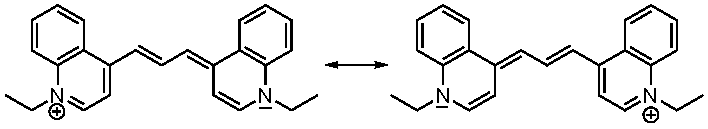
\includegraphics[width=0.8\linewidth]{../Abbildungen/11_4/Struktur_Cryptocyanin.pdf}
    \caption{Struktur von Cryptocyanin}
    \label{fig:struktur_carotin}
\end{figure}

Die mittlere Bindungslänge der zu betrachteten Bindungen beträgt $l = \SI{139.4}{\pico\metre}$. Die Masse eines Elektrons beträgt \SI{9.109e-31}{\kilo\gram}. Vernachlässige zur Berechnung der Länge des Kastens die Bindungswinkel im System.
\pagebreak
\teilaufgabe{\operator{Berechne} die Wellenlänge, bei der Kryptocyanin Licht absorbiert. \operator{Gib} die Farbe \operator{an}, die daraus resultiert.}{}
\kasten{105mm}{
Anzahl der Bindungen: $a = 10$\punkte{0.5}
\begin{align*}
    L &= l \cdot (a + 2) = \SI{139.4}{\pico\metre} \cdot 12 = \SI{1.6728}{\nano\metre}\punkte{1}\\
    \Delta E &= E_{7} - E_{6}\punkte{1.5} = \frac{h^2}{8\cdot m\cdot L^2}\cdot \left(7^2-6^2\right) = \frac{h^2}{8\cdot m\cdot L^2}\cdot 13
\intertext{\kommentar{Alternativ können auch beide Energien einzeln berechnet werden und danach die Differenz genommen werden. Halber Punkt für Differenz ziehen, je halber Punkt für richtiges Energieniveau.}}
    \Delta E &= \frac{\left(\SI{6.626e-34}{\joule\second}\right)^2}{8\cdot\SI{9.109e-31}{\kilo\gram}\cdot \left(\SI{1.6728}{\nano\metre}\right)^2}\cdot 13 = \SI{2.799e-19}{\joule}\punkte{1}\\
    \lambda &= \frac{h\cdot c}{\Delta E}\punkte{0.5}\\
    \lambda &= \frac{\SI{6.626e-34}{\joule\second} \cdot \SI{2.998e8}{\metre\per\second}}{\SI{2.799e-19}{\joule}} = \SI{7.097e-7}{\metre} \approx \SI{710}{\nano\metre}\punkte{1}
\end{align*}
Kryptocyanin absorbiert bei etwa \SI{710}{\nm} und damit rotes Licht, sodass es blau erscheint.\punkte{1}
}

\aufgabenende
\end{document}
